% ================================================================= HUẤN LUYỆN LẠI TRÊN 22 SẢN PHỤ
\subsection{Huấn luyện lại trên 22 sản phụ}
\label{sec:model22}

Mọi con số ở các mục trước đều từ mô hình học trên \textbf{5 ca chuyển dạ, 25 phút} dữ liệu. Nhóm đã huấn
luyện lại trên \textbf{22 sản phụ độc lập, 260 phút}: 5 PhysioNet, 7 Silesia B2 không trùng, và 10
Silesia B1 thai kỳ. Mã tại \texttt{model/train\_22.py} và \texttt{model/augment.py}.

\subsubsection{Giao thức}

Tách theo nhóm 11 fold, mỗi fold giữ lại 2 chủ thể (ghép một thai kỳ với một chuyển dạ khi có thể), một
chủ thể validation riêng có nhãn da đầu để chọn ngưỡng, 19 chủ thể huấn luyện. Tăng cường dữ liệu trên
từng đoạn khi huấn luyện, mỗi phép xác suất 0,5: nhân biên độ 0,7--1,4; cộng nhiễu Gauss ở SNR 10--30\,dB;
trôi đường nền hình sin 0,1--0,5\,Hz; dịch thời gian $\pm$100\,ms. Không tăng cường khi validation hay
test. Bốn epoch (ngân sách 190 phút CPU), seed 0. Sau 11 fold, mô hình production huấn luyện trên cả 22.

Nhóm tự kiểm tra rò rỉ trên metadata của từng checkpoint: 11 fold có ba tập rời nhau, 22 chủ thể mỗi
người đúng một lần, không có bản ghi nào trong nhóm 5 bản trùng PhysioNet. Một fold (fold 10) chọn
ngưỡng 0,20 --- cực đoan so với 0,65--0,80 của các fold khác; nhóm ghi nhận và không can thiệp.

\subsubsection{Kết quả trên 22 chủ thể}

\begin{table}[H]\centering\small
\caption{Mô hình 5 ca so với mô hình 22 ca trên cùng chủ thể và cùng kênh. Wilcoxon ghép cặp; ``thắng''
là số chủ thể mô hình 22 ca cao hơn.}
\label{tab:m22}
\begin{tabular}{@{}L{3.6cm} C{0.8cm} C{1.6cm} C{1.6cm} C{1.5cm} C{1.4cm} C{1.6cm} C{1.6cm} C{1.6cm}@{}}
\toprule
\textbf{Nhóm} & $n$ & \multicolumn{4}{c}{\textbf{Kênh PSD mù nhãn}} & \multicolumn{3}{c}{\textbf{Trung bình 4 kênh}} \\
\cmidrule(lr){3-6}\cmidrule(lr){7-9}
 & & \textbf{5 ca} & \textbf{22 ca} & $p$ & \textbf{thắng} & \textbf{5 ca} & \textbf{22 ca} & $p$ \\
\midrule
PhysioNet chuyển dạ & 5 & 99,21 & 99,40 & 1,00 & 2/2 & 97,45 & 98,69 & 0,24 \\
Silesia B2 chuyển dạ, ca mới & 7 & 95,87 & 96,82 & 0,125 & 4/0 & 93,73 & 94,50 & 0,016 \\
\textbf{Silesia B1 thai kỳ} & 10 & 93,30 & \tot{97,15} & \textbf{0,037} & \textbf{9/1} & 91,31 & \tot{97,01} & $<$\textbf{0,0001} \\
\midrule
\textbf{Toàn bộ} & 22 & 95,46 & \tot{97,56} & \textbf{0,007} & 15/3 & 93,47 & \tot{96,59} & $<$\textbf{0,0001} \\
\bottomrule
\end{tabular}
\end{table}

\begin{figure}[H]\centering
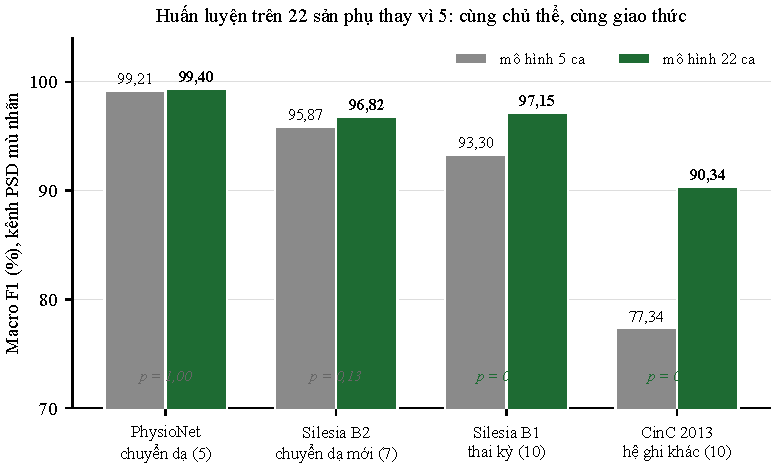
\includegraphics[width=0.9\textwidth]{figs/fig16_m22.pdf}
\caption{Cùng chủ thể, cùng giao thức, chỉ đổi mô hình. Lợi ích tập trung đúng ở hai chỗ yếu: thai kỳ
và hệ ghi khác.}
\label{fig:m22}
\end{figure}

Độ lệch chuẩn trên B1 giảm từ 13,46 xuống \textbf{4,95}. Hai ca thai kỳ khó nhất: B1\_07 từ 58,7 lên
\textbf{86,6}; B1\_06 từ 80,9 lên \textbf{89,5}. Trên PhysioNet, nơi mô hình 5 ca đã ở 99,21, không có khác
biệt có ý nghĩa --- đúng như kỳ vọng.

\begin{ghichu}[title={Kiểm tra nhãn B1 gián tiếp có kéo lệch mô hình không}]
Nhãn B1 lệch 8--12\,ms sau đỉnh R bụng ở 5/10 bản ghi và chiếm khoảng 72\% đoạn huấn luyện. Nếu mô hình
học theo ``phong cách nhãn B1'', nó sẽ lệch trên các ca có nhãn da đầu. Đo được: trung vị lệch (dự đoán
$-$ nhãn) của mô hình 22 ca trên PhysioNet là \textbf{0,0\,ms}, trên B2 là \textbf{0,0\,ms}, trên B1 là
$-1{,}0$\,ms. Không lệch.
\end{ghichu}

\subsubsection{Sụp đổ trên CinC 2013 được chữa phần lớn}

Đây là mục tiêu chưa đạt rõ nhất của bản trước. Mô hình production 22 ca chạy zero-shot trên CinC 2013 ---
hệ ghi khác, chưa từng thấy:

\begin{table}[H]\centering\small
\caption{Zero-shot trên CinC 2013 set-a, 10 bản ghi. Cùng giao thức, chỉ đổi mô hình.}
\label{tab:cinc22}
\begin{tabular}{@{}L{4.2cm} C{2.6cm} C{2.6cm} C{2.2cm} C{2.2cm}@{}}
\toprule
\textbf{Chỉ số} & \textbf{Mô hình 5 ca} & \textbf{Mô hình 22 ca} & \textbf{$p$ Wilcoxon} & \textbf{thắng/thua} \\
\midrule
Macro F1, kênh cố định & $77{,}34 \pm 28{,}54$ & $\mathbf{90{,}34 \pm 12{,}03}$ & \textbf{0,016} & 7/0 \\
Macro F1, kênh PSD & $59{,}15 \pm 37{,}17$ & $69{,}31 \pm 32{,}38$ & 0,031 & 6/1 \\
Macro F1, trung bình 4 kênh & $61{,}96 \pm 34{,}09$ & $72{,}64 \pm 25{,}76$ & 0,031 & 6/1 \\
Bản ghi F1 $\geq$ 90 (kênh cố định) & 5/10 & 6/10 & & \\
Bản ghi F1 $<$ 50 (kênh cố định) & \xau{3/10} & \tot{0/10} & & \\
\bottomrule
\end{tabular}
\end{table}

Từng bản ghi, kênh cố định: a02 từ 23 lên 76; a06 từ 43 lên 75; a10 từ 49 lên 71; a09 từ 80 lên 94.
\textbf{Phân bố lưỡng cực biến mất.}

\begin{canhbao}[title={Điều này sửa lại một kết luận của bản trước}]
Bản trước viết: ``biến gây sụp đổ là thiết bị và bố trí điện cực, không phải tuổi thai''. Phát biểu đó
đúng với mô hình 5 ca nhưng \textbf{thiếu một vế}. Với 22 ca --- vẫn cùng một bệnh viện, cùng một hệ ghi ---
mô hình chuyển sang hệ ghi khác ở mức 90 chứ không phải 77. Nghĩa là phần lớn sụp đổ đến từ \textbf{thiếu
dữ liệu}, và sự đa dạng giữa các sản phụ trong cùng một hệ ghi đã đủ để bù được phần lớn khác biệt phần
cứng. Khoảng cách còn lại (90 so với 97--99 trong miền) mới là phần thật sự do thiết bị.
\end{canhbao}

\subsubsection{Đường cong hiệu quả mẫu}

Vì sao 22 ca giúp nhiều đến vậy? Nhóm đo trực tiếp bằng cách huấn luyện trên $k$ sản phụ PhysioNet rồi
chấm trên những người còn lại.

\begin{figure}[H]\centering
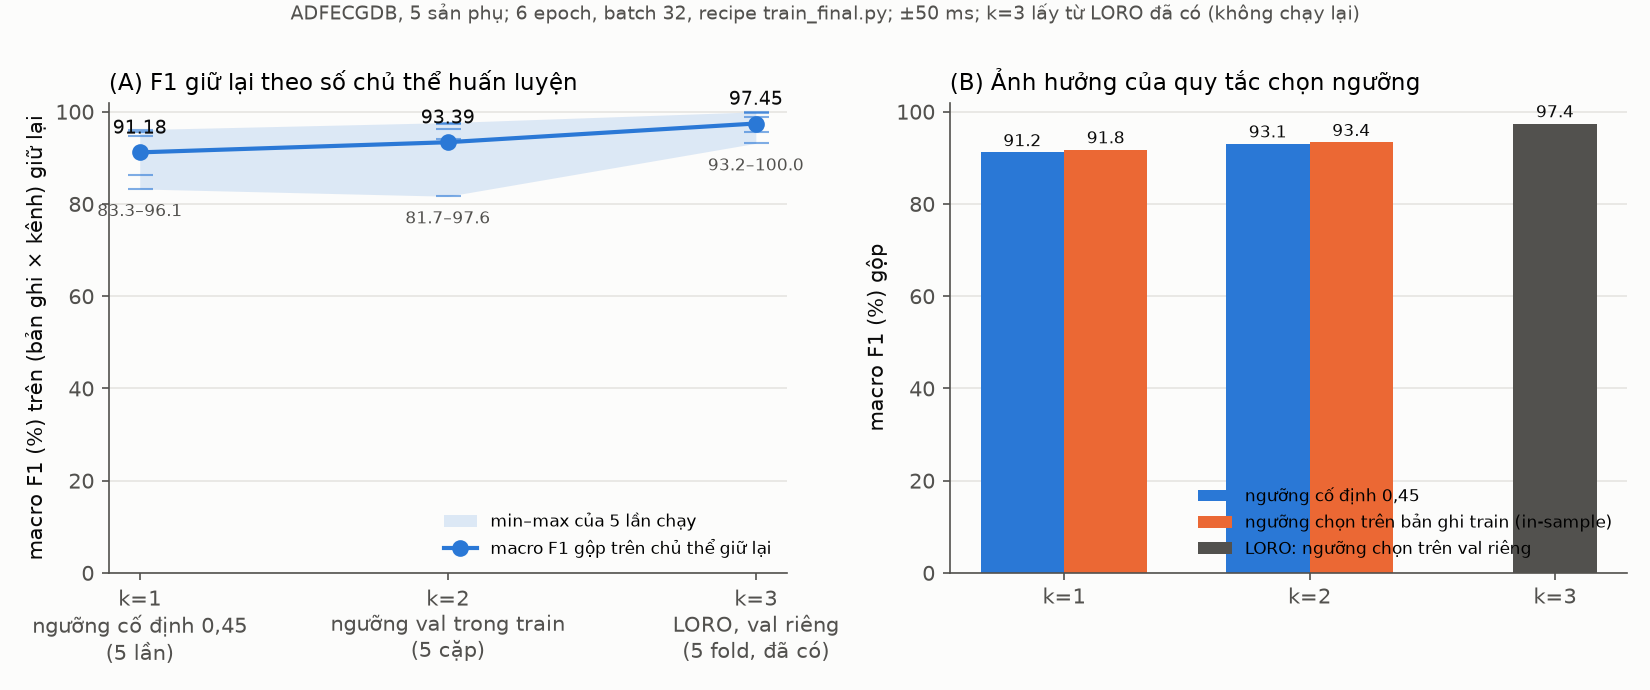
\includegraphics[width=0.96\textwidth]{figs/fig15_sample_efficiency.png}
\caption{(A) Macro F1 trên chủ thể giữ lại theo số chủ thể huấn luyện; dải mờ là min--max của 5 lần chạy.
(B) Ảnh hưởng của quy tắc chọn ngưỡng. Với $k = 1$ không có chủ thể validation nên dùng ngưỡng cố định
0,45; với $k = 2$ ngưỡng chọn trên một chủ thể trong tập huấn luyện --- cả hai đều được ghi rõ.}
\label{fig:sample_eff}
\end{figure}

\begin{table}[H]\centering\small
\caption{Hiệu quả mẫu trên ADFECGDB, 6 epoch, dung sai $\pm$50\,ms.}
\label{tab:sample_eff}
\begin{tabular}{@{}C{2.6cm} C{2.4cm} C{2.6cm} C{2.6cm} L{4.0cm}@{}}
\toprule
\textbf{Số ca huấn luyện} & \textbf{Số lần chạy} & \textbf{Macro F1 giữ lại} & \textbf{Min--max} & \textbf{Ngưỡng} \\
\midrule
1 & 5 & 91,18 & 83,3 -- 96,1 & cố định 0,45 \\
2 & 5 cặp & 93,39 & 81,7 -- 97,6 & trên một ca trong train \\
3 & 5 fold (tách bản ghi) & \textbf{97,45} & 93,2 -- 100,0 & trên ca validation riêng \\
\bottomrule
\end{tabular}
\end{table}

Đường cong \textbf{chưa bão hoà} ở 3 ca. Kết hợp với kết quả 22 ca, đây là bằng chứng định lượng cho luận
điểm xuyên suốt đề tài: trong bài toán này, đầu tư vào \textit{dữ liệu và front-end} sinh lợi hơn đầu tư
vào \textit{kiến trúc}.

\subsubsection{Giới hạn}

Một seed, bốn epoch (loss vẫn giảm ở epoch cuối). Chưa đo riêng đóng góp của tăng cường dữ liệu --- so sánh
``có'' và ``không'' tăng cường trên cùng fold là việc kế tiếp. Mô hình 22 ca chưa được chạy qua cổng tin
cậy học được; cổng đó hiệu chuẩn theo mô hình 5 ca. Fold 10 chọn ngưỡng 0,20, một điểm cần xem lại. Silesia
và PhysioNet cùng một bệnh viện, nên ``22 sản phụ'' vẫn là một trung tâm.
